\documentclass[12pt,letterpaper,titlepage,en-US]{article}

\usepackage{basicstyle}
\usepackage{report}
\usepackage{knit}
\usepackage{amsmath}
\usepackage{xcolor}
\usepackage{listings}
\usepackage{fancyvrb}
\usepackage{graphicx}

\definecolor{lbcolor}{rgb}{0.969, 0.969, 0.969} 

 \lstset{ 
    language=C++, % choose the language of the code
    basicstyle=\fontfamily{pcr}\selectfont\footnotesize\color{black},
    keywordstyle=\color{black}, % style for keywords
    numbers=none, % where to put the line-numbers
    numberstyle=\tiny, % the size of the fonts that are used for the line-numbers     
    backgroundcolor=\color{lbcolor},
    showspaces=false, % show spaces adding particular underscores
    showstringspaces=false, % underline spaces within strings
    showtabs=false, % show tabs within strings adding particular underscores
    frame=single, % adds a frame around the code
    tabsize=2, % sets default tabsize to 2 spaces
    rulesepcolor=\color{gray},
    rulecolor=\color{black},
    captionpos=b, % sets the caption-position to bottom
    breaklines=true, % sets automatic line breaking
    breakatwhitespace=false, 
}


\newcommand{\hmwkTitle}{Mini Project \#2}
\DTMsavetimestamp{DueDate}{2019-02-26T10:00:00-06:00}
\newcommand{\hmwkClass}{CS 6313.001}
\newcommand{\hmwkClassName}{Statistical Methods for Data Science}
\newcommand{\hmwkClassInstructor}{Instructor: Prof. Min Chen}
\newcommand{\hmwkAuthorName}{Shyam Patharla}
\newcommand{\hmwkAuthorNetID}{sxp178231}



%
% Title Page
%

\title{
    \vspace{1in}
    \textmd{\textbf{\hmwkClassName \\\hmwkClass:\ \hmwkTitle }}\\
     \normalsize\vspace{0.1in}\small{Due\ on\ \DTMusedate{DueDate}\ at \DTMusetime{DueDate} }\\
    \vspace{0.1in}\large{\textit{\hmwkClassInstructor}}\\
    \vspace{0.5in}
\includegraphics[height=2.4em]{UTD_logo_BW}\\
    \vspace{2in}
}

\author{\textbf{\hmwkAuthorName\ \footnotesize{(\hmwkAuthorNetID)}} \\ }
\date{}
\makeindex

\begin{document}
\maketitle

\pagenumbering{Roman}

\tableofcontents

\pagebreak
\pagenumbering{arabic}


\section{Answers}

\subsection{}
\subsubsection{Create a bar graph for the variable Maine}
\begin{enumerate}


\item Read the \emph{roadrace.csv} file.
\item Get the tuples of runners who are from Maine. Store them in the vector \textbf{from.maine}.
\item Get the tuples of runners who are not from Maine(Away). Store them in the vector \textbf{not.from.maine}.
\item Get the number of rows in from.maine and not.from.maine and store them in a vector.
\item Barplot the vector.
\end{enumerate}
We get the following barplot:
\begin{center}
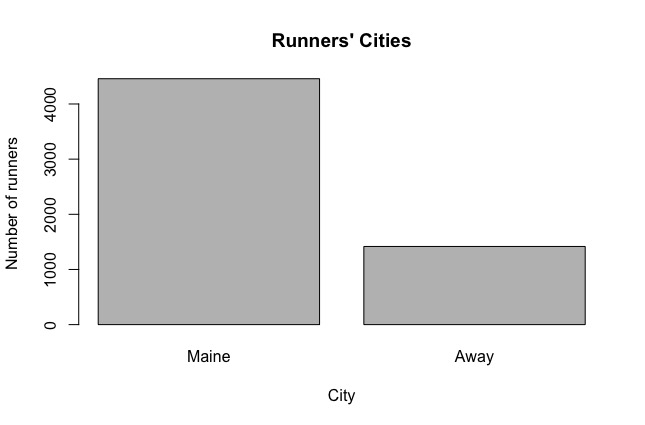
\includegraphics[scale=0.6]{1a.jpeg}
\end{center}

Inferences:
\begin{enumerate}
\item The number of runners from Maine is quite high compared to the number of Runners not form Maine.
\item The number of runners from Maine (4458) is cloose to thrice the number of runners not from Maine (1417).
\item This is reasonable since the number of participants from the city in which marathon is conducted is of often more.



\end{enumerate}

\subsubsection{Histograms for Runner's Times - Maine and Away}



\begin{enumerate}
\item We plot the histogram of the values in the 12th column of the \textbf{from.maine} vector i.e. the runners' time (minutes) for the runners from Maine.
\item We plot the histogram of the values in the 12th column of the \textbf{not.from.maine} vector i.e. the runners' time (minutes) for the runners not from Maine.
\end{enumerate}

We get the following two histograms:
\begin{center}
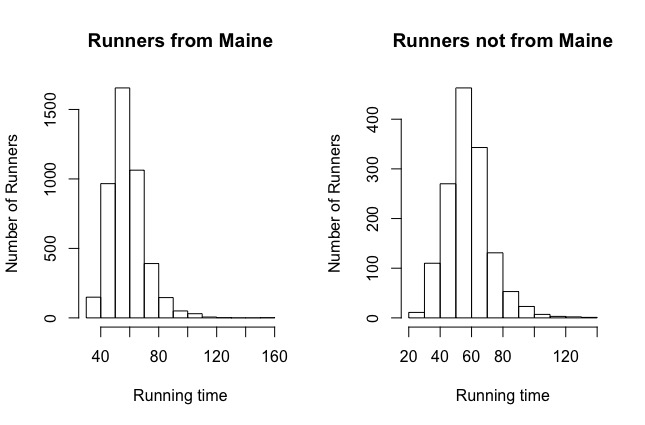
\includegraphics[scale=0.6]{1b.jpeg}
\end{center}

We can infer the follwing:
\begin{enumerate}
\item The histogram in the case of Maine runners looks right-skewed. It has 2 bars to the left of its highest bar and 5 bars to the right of its highest bar.
\item The histogram in the case of Maine runners, though it looks like a normal distribution, is also right-skewed.  It has 3 bars to the left of its highest bar and 5 bars to the right of its highest bar.
 
\item We can make more inferences after drawing the boxplots for the 2 cases as is shown in the next question.



\end{enumerate}

\subsubsection{Boxplots for Runners' Times - Maine and Away}
\begin{enumerate}
\item We boxplot the values in the 12th column of the \textbf{from.maine} vector i.e. the runners' time (minutes) for the runners from Maine.
\item We boxplot the values in the 12th column of the \textbf{not.from.maine} vector i.e. the runners' time (minutes) for the runners not from Maine.
\end{enumerate}
Without using the 1.5 * IQR rule, we get the following boxplot:
\begin{center}
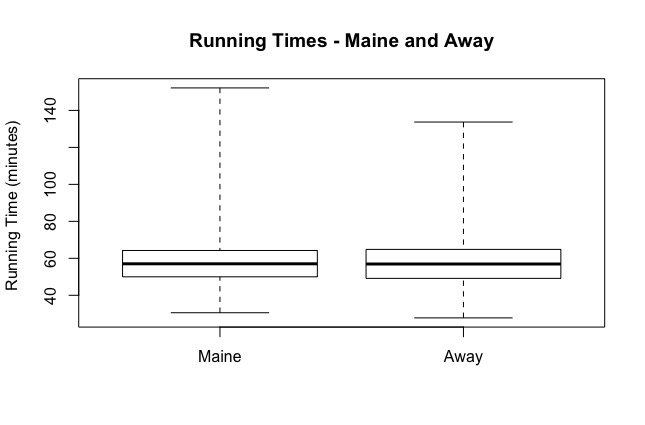
\includegraphics[scale=0.6]{1c2.jpeg}
\end{center}


Using the 1.5 * IQR rule, we get the following boxplot:
\begin{center}
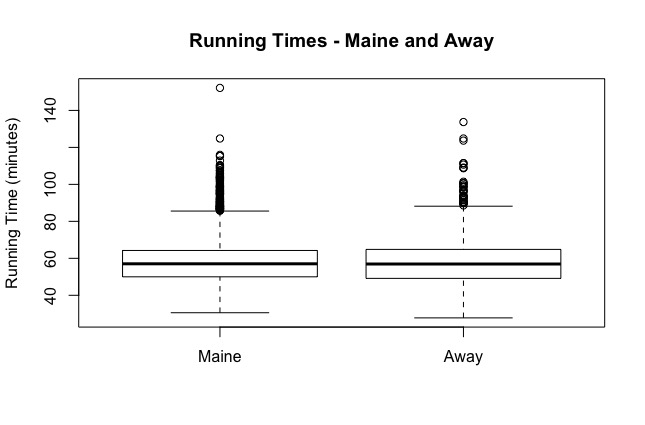
\includegraphics[scale=0.6]{1c.jpeg}
\end{center}


From the above boxplots, we can infer the following:

\begin{enumerate}

\item The Maine and Away distributions both have a \textbf{median} value close to 60 as the boxplots indicate. This is confirmed by:
\begin{knitrout}
\definecolor{shadecolor}{rgb}{0.969, 0.969, 0.969}\color{fgcolor}
\begin{kframe}

\begin{verbatim}
> median(from.maine[,12])
## [1] 57.0335

> median(not.from.maine[,12])
## [1] 56.92
\end{verbatim}
\end{kframe}
\end{knitrout}



\item The \textbf{quartiles} of the Maine Runners are close to their counterparts in the Away distribution. This is true since:

\begin{knitrout}
\definecolor{shadecolor}{rgb}{0.969, 0.969, 0.969}\color{fgcolor}
\begin{kframe}

\begin{verbatim}
> quantile(from.maine[,12])
##       0%       25%       50%       75%      100% 
## 30.56700  49.99550  57.03350  64.24325 152.16700 

> quantile(not.from.maine[,12])
##     0%     25%     50%     75%    100% 
## 27.782  49.153  56.920  64.827 133.710 
\end{verbatim}
\end{kframe}
\end{knitrout}




\item  The distribution for the Away runners has a slightly higher \textbf{inter-quartile range} (Q3 - Q1) in comparison to the distribution of the Maine runners. This is confirmed by the following:

\begin{knitrout}
\definecolor{shadecolor}{rgb}{0.969, 0.969, 0.969}\color{fgcolor}
\begin{kframe}

\begin{verbatim}
> quantile(from.maine[,12])[4]-quantile(from.maine[,12])[2]
##     75% 
## 14.24775 

> quantile(not.from.maine[,12])[4]-quantile(not.from.maine[,12])[2]
##   75% 
## 15.674 

\end{verbatim}
\end{kframe}
\end{knitrout}


\item The distribution for the Maine runners has a slightly higher \textbf{range} (highest value - lowest value) in comparison to the Away runners when the \emph{1.5 * IQR} rule is \textbf{not applied}.
\begin{knitrout}
\definecolor{shadecolor}{rgb}{0.969, 0.969, 0.969}\color{fgcolor}
\begin{kframe}

\begin{verbatim}
> quantile(from.maine[,12])[5]-quantile(from.maine[,12])[1]
##  100% 
##  121.6 

> quantile(not.from.maine[,12])[5]-quantile(not.from.maine[,12])[1]
##  100% 
##  105.928 
 
\end{verbatim}
\end{kframe}
\end{knitrout}



\item The distribution for the Away runners has a slightly higher \textbf{range} (highest value - lowest value) in comparison to the Maine runners when the \emph{1.5 * IQR rule} is \textbf{applied}.

\begin{knitrout}
\definecolor{shadecolor}{rgb}{0.969, 0.969, 0.969}\color{fgcolor}
\begin{kframe}

\begin{verbatim}
# Getting Q3 + 1.5 * IQR for Maine
> high <- 1.5 * (quantile(from.maine[,12])[4] - 
quantile(from.maine[,12])[2]) + quantile(from.maine[,12])[4]
##     75% 
## 85.61487 

# Getting Q1 - 1.5 * IQR for Maine
> low <- 1.5 *( quantile(from.maine[,12])[4] - 
quantile(from.maine[,12])[2])*(-1)+ quantile(from.maine[,12])[2]
##    75% 
## 28.62388 

# Range for Running times of Maine runners
> high - low
##  56.99099



# Getting Q3 + 1.5 * IQR for Away
> high <- 1.5 * (quantile(from.maine[,12])[4] - 
quantile(not.from.maine[,12])[2]) + quantile(not.from.maine[,12])[4]
##     75% 
## 	88.338  

# Getting Q1 - 1.5 * IQR for Away
> low <- 1.5 *( quantile(from.maine[,12])[4] - 
quantile(not.from.maine[,12])[2])*(-1)+ quantile(not.from.maine[,12])[2]
##    75% 
##   25.642 

# Range for Running times of Away runners
> high-low
##   75% 
## 62.696 

\end{verbatim}
\end{kframe}
\end{knitrout}


\item The distribution for Maine Runners has far more \textbf{outliers} than in the case of Away Runners.

\item Most of the outliers in both boxplots are close to the (Q3 + 1.5 * IQR) value.

\item The outliers are only on the \textbf{higher end} of the distribution and not the lower end in both cases.



\item The \textbf{standard deviation} of the Away Runners' distribution is slightly higher than that of the Maine Runners' distribution:
\begin{knitrout}
\definecolor{shadecolor}{rgb}{0.969, 0.969, 0.969}\color{fgcolor}
\begin{kframe}

\begin{verbatim}
> sd(from.maine[,12])
## [1] 12.18511

> sd(not.from.maine[,12])
## [1] 13.83538
\end{verbatim}
\end{kframe}
\end{knitrout}



\item The Maine distribution has a \textbf{mean} value slightly larger than that of the Away distribution. This is true since:

\begin{knitrout}
\definecolor{shadecolor}{rgb}{0.969, 0.969, 0.969}\color{fgcolor}
\begin{kframe}

\begin{verbatim}
> mean(from.maine[,12])
## [1] 58.19514

> mean(not.from.maine[,12])
## [1] 57.82181

\end{verbatim}
\end{kframe}
\end{knitrout}

\end{enumerate}





\subsubsection{Boxplots for Runners' Ages - Male and Female}
\begin{enumerate}
\item Read the \emph{roadrace.csv} file.
\item Get the tuples of runners who are males. Store them in the vector \textbf{male.runners}.
\item Get the tuples of runners who are females. Store them in the vector \textbf{female.runners}.
\item We boxplot the values in the 12th column of the \textbf{male.runners} vector.
\item We boxplot the values in the 12th column of the \textbf{female.runners} vector.
\end{enumerate}
Without using the 1.5 * IQR rule, we get the following boxplot:
\begin{center}
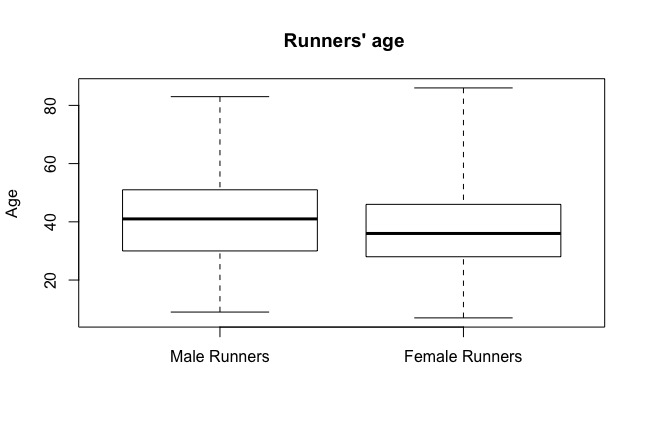
\includegraphics[scale=0.6]{1d2.jpeg}
\end{center}


Using the 1.5 * IQR rule, we get the following boxplot:
\begin{center}
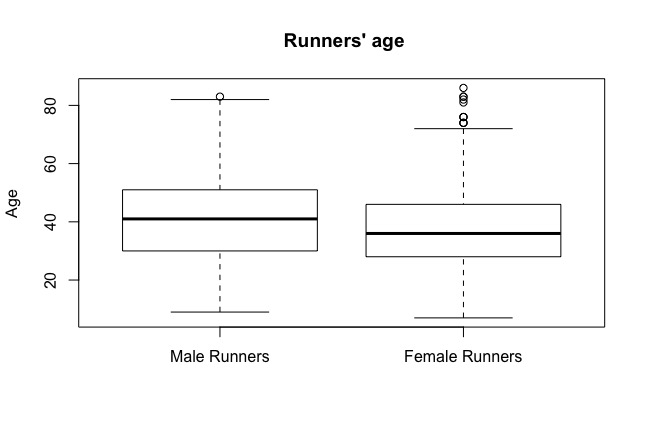
\includegraphics[scale=0.6]{1d.jpeg}
\end{center}


From the above boxplots, we can infer the following:

\begin{enumerate}

\item The male runners' age distribution has a higher \textbf{median} in comparison to that of the female runners'. This is confirmed by:
\begin{knitrout}
\definecolor{shadecolor}{rgb}{0.969, 0.969, 0.969}\color{fgcolor}
\begin{kframe}

\begin{verbatim}
> median(male.runners[,5])
## [1] 41
 
> median(female.runners[,5])
## [1] 36
\end{verbatim}
\end{kframe}
\end{knitrout}



\item The \textbf{quartiles} of the male runners' age distribution are close to their counterparts in the female runners' age distribution. This is true since:

\begin{knitrout}
\definecolor{shadecolor}{rgb}{0.969, 0.969, 0.969}\color{fgcolor}
\begin{kframe}

\begin{verbatim}
> quantile(male.runners[,5])
##  0%  25%  50%  75% 100% 
##  9   30   41   51   83 
   
> quantile(female.runners[,5])
##   0%  25%  50%  75% 100% 
##   7   28   36   46   86 
\end{verbatim}
\end{kframe}
\end{knitrout}




\item  The distribution for the male runners' ages has a higher \textbf{inter-quartile range} (Q3 - Q1) in comparison to the age distribution of the female runners. This is confirmed by the following:

\begin{knitrout}
\definecolor{shadecolor}{rgb}{0.969, 0.969, 0.969}\color{fgcolor}
\begin{kframe}

\begin{verbatim}
> quantile(male.runners[,5])[4] - quantile(male.runners[,5])[2]
## 75% 
##  21 
 
> quantile(female.runners[,5])[4] - quantile(female.runners[,5])[2]
## 75% 
## 18 
\end{verbatim}
\end{kframe}
\end{knitrout}


\item The distribution for the male runners has a slightly lower \textbf{range} (highest value - lowest value) in comparison to female runners when the \emph{1.5 * IQR} rule is \textbf{not applied}.
\begin{knitrout}
\definecolor{shadecolor}{rgb}{0.969, 0.969, 0.969}\color{fgcolor}
\begin{kframe}

\begin{verbatim}
# Range for male runners' ages
> quantile(male.runners[,5])[5] - quantile(male.runners[,5])[1]
## 100% 
##  74 
  
# Range for female runners' ages
> quantile(female.runners[,5])[5] - quantile(female.runners[,5])[1]
## 100% 
##  79 
\end{verbatim}
\end{kframe}
\end{knitrout}



\item The age distribution for male runners has a slightly higher \textbf{range} (highest value - lowest value) in comparison to that of female runners when the \emph{1.5 * IQR rule} is \textbf{applied}.

\begin{knitrout}
\definecolor{shadecolor}{rgb}{0.969, 0.969, 0.969}\color{fgcolor}
\begin{kframe}
\begin{verbatim}
# Getting Q3 + 1.5 * IQR for males
> high <- 1.5 * (quantile(male.runners[,5])[4] -
quantile(male.runners[,5])[2]) + quantile(male.runners[,5])[4]
##     75% 
## 82.5

# Getting Q1 - 1.5 * IQR for males
> low <- 1.5 * (quantile(male.runners[,5])[4] -
quantile(male.runners[,5])[2])*(-1) + quantile(male.runners[,5])[2]
##    75% 
## -1.5

# Range for Running times of male runners
> high - low
##  84


# Getting Q3 + 1.5 * IQR for females
> high <- 1.5 * (quantile(female.runners[,5])[4] -
quantile(female.runners[,5])[2]) + quantile(female.runners[,5])[4]
##   75% 
##  73 

# Getting Q1 - 1.5 * IQR for females
> low <- 1.5 * (quantile(female.runners[,5])[4] -
quantile(female.runners[,5])[2])*(-1) + quantile(female.runners[,5])[2]
##  75% 
##   1 

# Range for Running times of female runners
> high-low
##  75% 
## 72
\end{verbatim}
\end{kframe}
\end{knitrout}


\item The age distribution for female runners has far more \textbf{outliers} than in the case of male runners.

\item The outliers are only on the \textbf{higher end} of the distribution and not the lower end.


\item The \textbf{standard deviation} of the male runners' ages is slightly higher than that of the female runners' distribution.
\begin{knitrout}
\definecolor{shadecolor}{rgb}{0.969, 0.969, 0.969}\color{fgcolor}
\begin{kframe}

\begin{verbatim}
> sd(male.runners[,5])
## [1] 13.99289

> sd(female.runners[,5])
## [1] 12.26925
\end{verbatim}
\end{kframe}
\end{knitrout}



\item The male runners' age distribution has a \textbf{mean} value slightly larger than that of the female runners's age distribution. This is true since:

\begin{knitrout}
\definecolor{shadecolor}{rgb}{0.969, 0.969, 0.969}\color{fgcolor}
\begin{kframe}

\begin{verbatim}
> mean(male.runners[,5])
## [1] 40.4468
> mean(female.runners[,5])
## [1] 37.23653
\end{verbatim}
\end{kframe}
\end{knitrout}

\end{enumerate}




\subsection{Boxplot for motorycle accidents in South Carolina}

\begin{enumerate}
\item Read the \emph{motorcycle.csv} file.

\item Boxplot the values the second column.
\end{enumerate}

We get the following boxplot:
\begin{center}
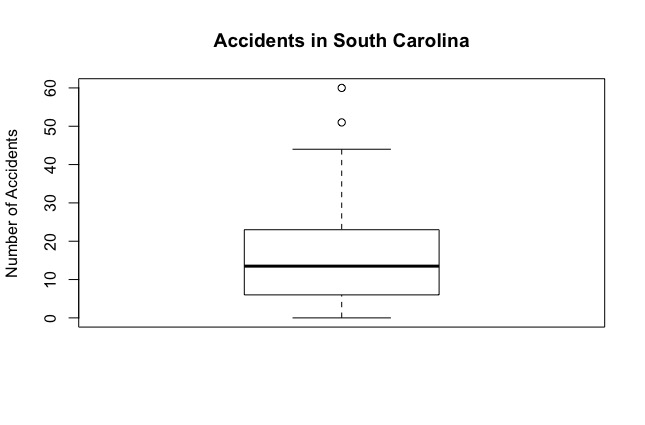
\includegraphics[scale=0.6]{2.jpeg}
\end{center}




We can infer the following:
\begin{enumerate}
\item The data  clearly has a \textbf{right skewed} distribution since there are more values at the right end.


\item The \textbf{mean} is higher than the \textbf{median}, as implied by the right-skewedness of the distribution.
\begin{knitrout}
\definecolor{shadecolor}{rgb}{0.969, 0.969, 0.969}\color{fgcolor}
\begin{kframe}

\begin{verbatim}
> mean (motorcycle[,2])
## [1] 17.02083

> median(motorcyle[,2])
## [1] 13.5
\end{verbatim}
\end{kframe}
\end{knitrout}


\item The \textbf{quartiles} also show the right-skewedness of the data since the first 3 quartiles are close to each other and there is a huge gap between the 3rd and 4th quartiles.

\begin{knitrout}
\definecolor{shadecolor}{rgb}{0.969, 0.969, 0.969}\color{fgcolor}
\begin{kframe}

\begin{verbatim}
> quantile(motorcycle[,2])
##  0%  25%  50%  75% 100% 
## 0.0  6.0 13.5 23.0 60.0 
\end{verbatim}
\end{kframe}
\end{knitrout}

\item The data has an \textbf{inter-quartile range} (Q3 - Q1) of 19.

\begin{knitrout}
\definecolor{shadecolor}{rgb}{0.969, 0.969, 0.969}\color{fgcolor}
\begin{kframe}

\begin{verbatim}
> quantile(motorcycle[,2])[4] - quantile(motorcycle[,2])[2]
##  75%
## 19
\end{verbatim}
\end{kframe}
\end{knitrout}


 \item The distribution has a \textbf{range} (highest value - lowest value) of 60 when the \emph{1.5 * IQR} rule is \textbf{not applied}.
\begin{knitrout}
\definecolor{shadecolor}{rgb}{0.969, 0.969, 0.969}\color{fgcolor}
\begin{kframe}

\begin{verbatim}
# Range for  number of accidents
> quantile(motorcycle[,2])[5] - quantile(motorcycle[,2])[1]
## 100% 
##  60
  
\end{verbatim}
\end{kframe}
\end{knitrout}



\item The distribution has a slightly higher \textbf{range} (highest value - lowest value) of 68 when the \emph{1.5 * IQR} rule is \textbf{applied}.

\begin{knitrout}
\definecolor{shadecolor}{rgb}{0.969, 0.969, 0.969}\color{fgcolor}
\begin{kframe}

\begin{verbatim}
> high <- 1.5*(quantile(motorcycle[,2])[4]-
quantile(motorcycle[,2])[2])+quantile(motorcycle[,2])[4]
## 75%
## 48.5

> low <- -1.5*(quantile(motorcycle[,2])[4]-
quantile(motorcycle[,2])[2])+quantile(motorcycle[,2])[2]
## 75%
## -19.5

> high - low
## 75% 
## 68 
\end{verbatim}
\end{kframe}
\end{knitrout}


 \item The distribution has a \textbf{standard deviation} of around 13.
\begin{knitrout}
\definecolor{shadecolor}{rgb}{0.969, 0.969, 0.969}\color{fgcolor}
\begin{kframe}

\begin{verbatim}
> sd(motorcycle[,2])
## 100% 
## [1] 13.81256  
\end{verbatim}
\end{kframe}
\end{knitrout}



\item There are 2 counties which are outliers:
\begin{enumerate}
\item Greenville, with 51 accidents
\item Horry, with 60 accidents
\end{enumerate}
\end{enumerate}






\section{R Code}

\lstinputlisting{/users/psprao/downloads/stats/R-code/project2/Q1.R}
\lstinputlisting{/users/psprao/downloads/stats/R-code/project2/Q2A.R}
\lstinputlisting{/users/psprao/downloads/stats/R-code/project2/Q2B.R}
\end{document}
